
% ----------------------------------------------------------------------
%  Set the document class
% ----------------------------------------------------------------------
\documentclass[11pt,a4paper,twoside]{article}

% ----------------------------------------------------------------------
% Define external packages, language, margins, fonts and new commands
% ----------------------------------------------------------------------
%\input{preamble} 
\usepackage[utf8]{inputenc}   % <<<<< Linux
\usepackage[english]{babel} % <<<<< English
\usepackage{notoccite}
\usepackage[skip=0.5\baselineskip]{caption}
\hyphenation{GTKWave}
\usepackage{listings}
\usepackage[all]{nowidow}
\usepackage{tabularx}
\usepackage{amsmath}
\usepackage{float}
\usepackage[pdf]{pstricks}

%blind text
\usepackage{lipsum}

\usepackage{graphicx}
\graphicspath{ {./} {../../figlib/} }
\def\FontLn{% 16 pt normal
  \usefont{T1}{phv}{m}{n}\fontsize{16pt}{16pt}\selectfont}
\def\FontLb{% 16 pt bold
  \usefont{T1}{phv}{b}{n}\fontsize{16pt}{16pt}\selectfont}
\def\FontMn{% 14 pt normal
  \usefont{T1}{phv}{m}{n}\fontsize{14pt}{14pt}\selectfont}
\def\FontMb{% 14 pt bold
  \usefont{T1}{phv}{b}{n}\fontsize{14pt}{14pt}\selectfont}
\def\FontSn{% 12 pt normal
  \usefont{T1}{phv}{m}{n}\fontsize{12pt}{12pt}\selectfont}

% Use Arial font as default
%
\renewcommand{\rmdefault}{phv}
\renewcommand{\sfdefault}{phv}
\usepackage{geometry}	
\geometry{verbose,tmargin=2.5cm,bmargin=2.5cm,lmargin=2.5cm,rmargin=2.5cm}

%\usepackage{setspace}
%\renewcommand{\baselinestretch}{1.5}

\usepackage[pdftex]{hyperref} % enhance documents that are to be
                              % output as HTML and PDF
\hypersetup{colorlinks,       % color text of links and anchors,
                              % eliminates borders around links
%            linkcolor=red,    % color for normal internal links
            linkcolor=black,  % color for normal internal links
            anchorcolor=black,% color for anchor text
%            citecolor=green,  % color for bibliographical citations
            citecolor=black,  % color for bibliographical citations
%            filecolor=magenta,% color for URLs which open local files
            filecolor=black,  % color for URLs which open local files
%            menucolor=red,    % color for Acrobat menu items
            menucolor=black,  % color for Acrobat menu items
%            pagecolor=red,    % color for links to other pages
            pagecolor=black,  % color for links to other pages
%            urlcolor=cyan,    % color for linked URLs
            urlcolor=black,   % color for linked URLs
	          bookmarks=true,         % create PDF bookmarks
	          bookmarksopen=false,    % don't expand bookmarks
	          bookmarksnumbered=true, % number bookmarks
	          pdftitle={report},
            pdfauthor={Andre C. Marta},
%            pdfsubject={Thesis Title},
%            pdfkeywords={Thesis Keywords},
            pdfstartview=FitV,
            pdfdisplaydoctitle=true}

\usepackage[numbers,sort&compress]{natbib} % <<<<< References in numbered list [1],[2],...
\usepackage{subcaption} 
\usepackage{mdframed}

%%%%%%%%%%%%%%%%%%%%%%%%%%%%%%%%%%%%%%%%%%%%%%%%%%%%%%%%%%%%%%%%%%%%%%%%
%     Begin Document                                                   %
%%%%%%%%%%%%%%%%%%%%%%%%%%%%%%%%%%%%%%%%%%%%%%%%%%%%%%%%%%%%%%%%%%%%%%%%


\begin{document}

% Set plain page style (no headers, footer with centered page number)
\pagestyle{plain}

% Set roman numbering (i,ii,...) before the start of chapters
%\pagenumbering{roman}

% ----------------------------------------------------------------------
%  Cover page
% ----------------------------------------------------------------------
%%%%%%%%%%%%%%%%%%%%%%%%%%%%%%%%%%%%%%%%%%%%%%%%%%%%%%%%%%%%%%%%%%%%%%%%
%                                                                      %
%     File: Thesis_FrontCover.tex                                      %
%     Tex Master: Thesis.tex                                           %
%                                                                      %
%     Author: Andre C. Marta                                           %
%     Last modified :  2 Jul 2015                                      %
%                                                                      %
%%%%%%%%%%%%%%%%%%%%%%%%%%%%%%%%%%%%%%%%%%%%%%%%%%%%%%%%%%%%%%%%%%%%%%%%

\thispagestyle {empty}


% IST Logo - Signature A
% parameters: bb=llx lly urx ury (bounding box), width=h_length, height=v_length, angle=angle, scale=factor, clip=true/false, draft=true/false. 
\includegraphics[bb=9.5cm 11cm 0cm 0cm,scale=0.29]{IST_A_CMYK_POS}

\begin{center}
%
% Figure (Image or plot)
\vspace{1.0cm}
% height = 50 mm
%\includegraphics[height=50mm]{Figures/Airbus_A350.jpg}

% Title, author and degree
\vspace{1cm}
{\FontLb Circuit Theory and Electronics Fundamentals} \\ % <<<<< EDIT TITLE
\vspace{1cm}
{\FontSn Aerospace Engineering, Técnico, University of Lisbon} \\ % <<<<< EDIT COURSE
\vspace{1cm}
{\FontSn 4\textsuperscript{th} Laboratory Report} \\
\vspace{1cm}
{\FontSn João Martins 95806} \\
{\FontSn Gonçalo Martins 95793}\\
{\FontSn António Lopes 95771}\\
\vspace{1cm}
{\FontSn May 23, 2021} \\ % <<<<< EDIT DATE (corresponds to date of oral examination)
%
\end{center}










% ----------------------------------------------------------------------
% Dedication page (optional)
% ----------------------------------------------------------------------
%\input{dedication} 
%\cleardoublepage

% ----------------------------------------------------------------------
%  Acknowledgments (optional)
% ----------------------------------------------------------------------
%\input{acknowledgements}
%\cleardoublepage

% ----------------------------------------------------------------------
%  Abstract (both in English and Portuguese)
% ----------------------------------------------------------------------
%\input{resumo} 
%\cleardoublepage

%\input{abstract} 

% ----------------------------------------------------------------------
%  Table of contents, list of tables, list of figures and nomenclature
% ----------------------------------------------------------------------

% Table of contents
%
\tableofcontents

% List of tables
%\addcontentsline{toc}{section}{\listtablename}
%\listoftables
%\cleardoublepage 

% List of figures
%\addcontentsline{toc}{section}{\listfigurename}
%\listoffigures
%\cleardoublepage 

% Set arabic numbering (1,2,...) after preface
%
%\setcounter{page}{1}
%\pagenumbering{arabic}

% ----------------------------------------------------------------------
%  Body
% ----------------------------------------------------------------------
\newpage
\section{Introduction}
\label{sec:introduction}

% state the learning objective 
The objective of this laboratory assignment is to study a circuit containing a
sinusoidal voltage source $V_I$ connected to a resistor $R$ and a capacitor $C$
in series. The circuit can be seen if Figure~\ref{fig:rc}.

\lipsum[1-1]

In Section~\ref{sec:analysis}, a theoretical analysis of the circuit is
presented. In Section~\ref{sec:simulation}, the circuit is analysed by
simulation, and the results are compared to the theoretical results obtained in
Section~\ref{sec:analysis}. The conclusions of this study are outlined in
Section~\ref{sec:conclusion}.

\begin{figure}[h] \centering
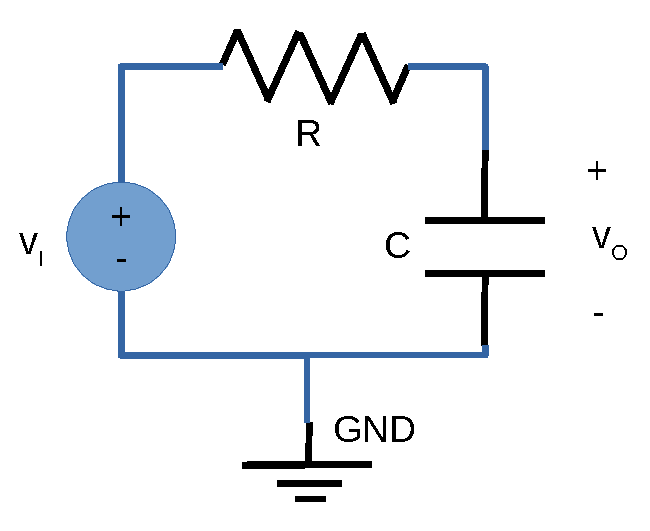
\includegraphics[width=0.4\linewidth]{rc.pdf}
\caption{Voltage driven serial RC circuit.}
\label{fig:rc}
\end{figure}


\newpage
\section{Theoretical Analysis}
\label{sec:theoretical}

\par In this section, the circuit shown in figure \ref{fig:1} is analysed theoretically.
\par Like we said in section \ref{sec:introduction}, both of the stages of the amplifier are going to be analysed in a more detailed way in this section.
\par Let's begin with the gain stage. The gain stage consists of a common emitter amplifier, with a NPN transistor, which allows us to obtain a high input impedance ($Z_{i_1}$), and a high gain $A_V$. However, this type of amplifier has a very high output impedance ($Z_{o_1}$), which causes a degeneration of the signal output. In order to solve this problem, the gain stage is connected to an output stage, which consists of a common collector amplifier, whith a PNP transistor. This stage has a gain a little bit lower than 1, but still very close to 1, and a very high input impedance ($Z_{o_2}$), which preserve the high gain of the previous stage. In addition, this circuit has a very low output impedance ($Z_{o_2}$), which means that almost all the gain is going to be delivered to the speaker.

\subsection{First Point}

\par Our theoretical analysis starts by computing the operating point, using the theoretical DC model studied. In order to do this, we harnessed the mesh method provided in the Octave script to which we added the new components.
\par The values of currents are presented in table \ref{tab:currents}, as well as the values of $V_{CE}$ and $V_{BE}$, and $V_{EC}$ and $V_{EB}$, respectively for the NPN and the PNP transistors, in order to prove that they're working in the forward active region ($V_{CE} > V_{BEON}$ and $V_{EC} > V_{EBON}$).


\vspace{5mm}
\begin{table}[H]
	\centering
	\begin{tabularx}{0.9\textwidth} {
 	    | >{\raggedright\arraybackslash}X
  	    | >{\raggedleft\arraybackslash}X | }
	\hline
	Low Cut Off & 9.090909e+03 rad/s\\ \hline
High Cut Off & 4.545455e+03 rad/s\\ \hline
Medio & 6.428243e+03 rad/s\\ \hline
Input Impedance & 1.000000e+03 \\ \hline
Output Impedance & 3.333333e+02 \\ \hline
Gain & 3.366667e+01 \\ \hline
Gain & 3.054400e+01 dB \\ \hline

	\end{tabularx}
	\caption{$V_{CE}$, $V_{BE}$, $V_{EC}$, $V_{EB}$, and circulation current values}
	\label{tab:currents}
\end{table}
\vspace{5mm}

\subsection{Second Point}

\par The second point in this analysis consists in computing the gain and input and output impedances separately for each stage.
\par In order to do this kind of analysis we have to consider the incremental model of the circuit.


\par In order to compute the gain of each stage, we used the formulae which were taught in the theoretical classes (which were also given in advance in Octave's script). We can use this simplified formulae, because we are assuming medium/high frequencies. Based on this assumption, we can replace the capacitor with a short circuit.
\par In a similar way, we computed the input and output impedances, using the formulae given in the theoretical classes (which were also given in advance in Octave's script), which are based on the same assumption.
\par To make things a little bit more clear, the input/output impedances are determined by connecting, for example, a voltage source to the stage's input/output and replacing the output/input with a short circuit. By determining the current that flows across the added voltage source, we can determine the input/output impedance by just applying Ohm's law. This values are shown in tables 2 and 3, respectively for the input and the output stages. The overall output impedance and gain are shown in table 4.

\vspace{5mm}
\begin{table}[H]
	\centering
	\begin{tabularx}{0.9\textwidth} {
 	    | >{\raggedright\arraybackslash}X
  	    | >{\raggedleft\arraybackslash}X | }
	\hline
	AV1dB & 3.158539e+01 dB\\ \hline
ZI1 & 2.419648e+03 Omega \\ \hline
ZO1 & 4.652785e+03 Omega \\ \hline

	\end{tabularx}
	\caption{Gain, input and output impedances - gain stage}
	\label{tab:stage1}
\end{table}
\vspace{5mm}

\begin{table}[H]
	\centering
	\begin{tabularx}{0.9\textwidth} {
 	    | >{\raggedright\arraybackslash}X
  	    | >{\raggedleft\arraybackslash}X | }
	\hline
	AV2dB & -9.207782e-02 dB\\ \hline
ZI2 & 7.218471e+04 Omega \\ \hline
ZO2 & 3.313468e+00 Omega \\ \hline

	\end{tabularx}
	\caption{Gain, input and output impedances - output stage}
	\label{tab:stage2}
\end{table}
\vspace{5mm}

\begin{table}[H]
	\centering
	\begin{tabularx}{0.9\textwidth} {
 	    | >{\raggedright\arraybackslash}X
  	    | >{\raggedleft\arraybackslash}X | }
	\hline
	AVdB & 3.120876e+01 dB\\ \hline
ZO & 2.270796e+01 Omega\\ \hline

	\end{tabularx}
	\caption{Overal gain and output impedance}
	\label{tab:overall}
\end{table}
\vspace{5mm}

\par As one might observe, the input impedance of the output stage ($Z_{i_2}$) is substantially greater than the output impedance of the gain stage ($Z_{o_1}$). Hence, because the voltage divider applied at the input of the output stage is given by

\begin{equation}
	v_{i_2}= \frac{Z_{i_2}}{Z_{o_1}+Z_{i_2}} \cdot v_{o_1}
\end{equation}

\noindent if $Z_{o_1}<<Z_{i_2}$, we can say that $v_{i_2} \approx v_{o_1}$. It's worth to mention that the gain of the output stage is approximately 1, so overall there is no significant signal loss when the two stages are put together.

\begin{equation}
	AV2dB = -9.207782e-02 \Rightarrow AV2 = 0.989455 \approx 1
\end{equation}

\subsection{Third Point}

\par The third point of this theoretical analysis is to compute the frequency responce $\frac{V_o(f)}{V_i(f)}$. 
\par In order to do so, we can't neglect the effect of the capacitors, since only this component's impedance is frequency dependent.
\par Being that, we calculated the transfer function of the circuit. To do that we calculated the two poles, the lower and high cut off frequency based on the document provided by the professor. Knowing that we built our transfer function and plotted the following figure.

\begin{figure}[H] 
	\centering
	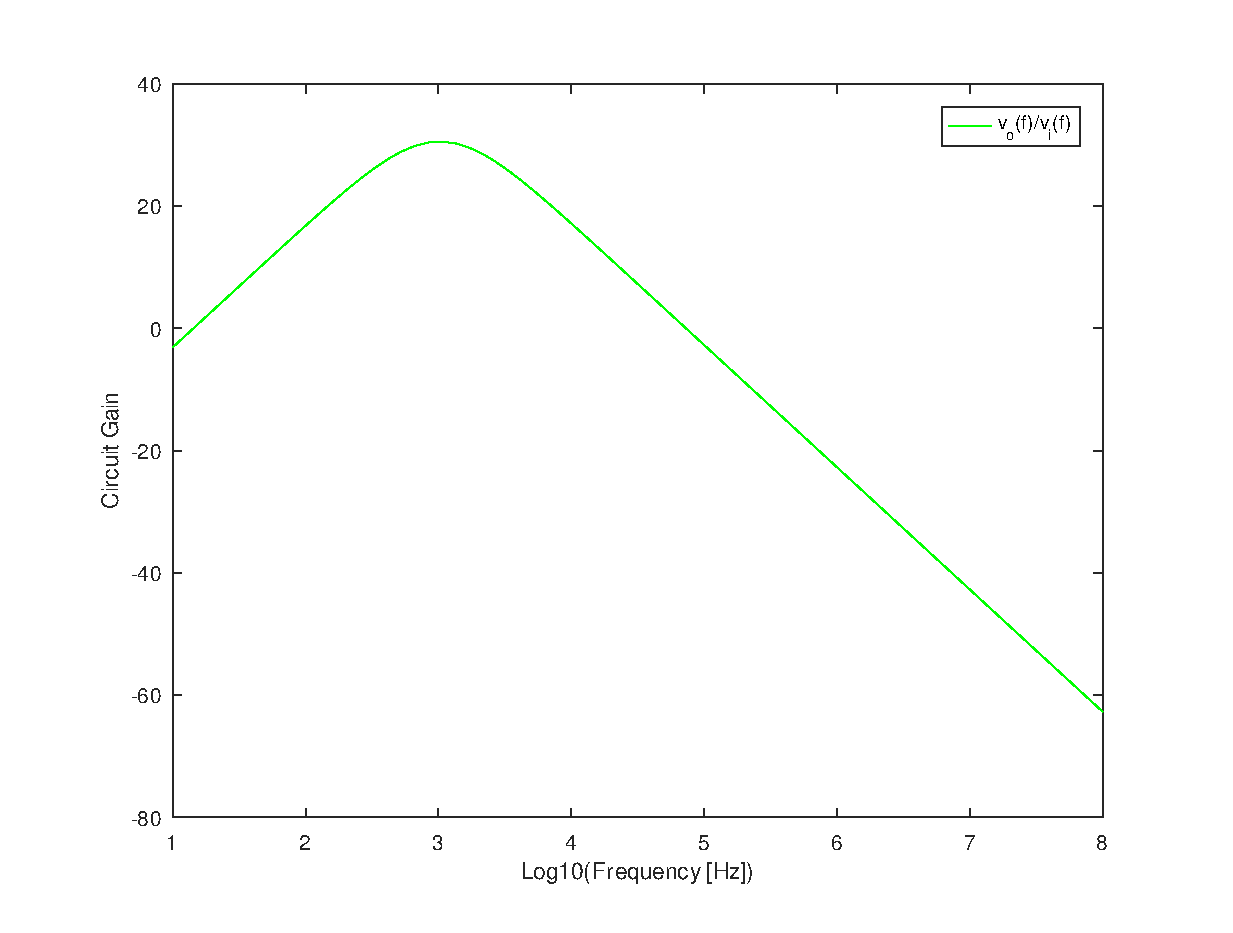
\includegraphics[width=1\linewidth]{teoria.eps}
	\caption{Frequency response of the amplifier ($\frac{V_o(f)}{V_i(f)}$)}
\end{figure}

\par Finally, the theoretical merit is shown below, as well as the high and low cutoff frequencies, the cost and the bandwidth.

\vspace{5mm}
\begin{table}[H]
	\centering
	\begin{tabularx}{0.9\textwidth} {
 	    | >{\raggedright\arraybackslash}X
  	    | >{\raggedleft\arraybackslash}X | }
	\hline
	Merit & 4.921738e+02 \\ \hline
HighCutOff frequency & 4.377991e+05 Hz\\ \hline
LowCutOff frequency & 1.262427e+01 Hz\\ \hline
Cost & 2.198943e+03 MU's\\ \hline
Bandwidth & 4.377865e+05 Hz\\ \hline
Max Gain & 3.111556e+01 V\\ \hline

	\end{tabularx}
	\caption{Theoretical variables of merit}
	\label{tab:merit1}
\end{table}
\vspace{5mm}


\newpage
\section{Simulation}
\label{sec:simulation}

\par In this section, a briet description of the circuit modeled through NGspice is going to be presented and the values obtained on it are going to be compared with the ones obtained on octave. The purpose of the simulation was to maximise the merit obtained and, as such, to obtain the values of the gain, bandwidth and the lower and higher  cut off frequencies as well as the input and output impedances.

\par In order to do that, the circuit in study was modelled in the program. For that, transistors of the given models (NPN transistor for the gain stage and PNP transistor for the output stage) were used on the two common amplifiers and the rest of the components specifications changed to be on par with the values optimised through the Matlab software (Simulink) and as seen in the octave sript.

\par With the circuit described, the next step was to analyse the simulations with the introduced values. The first step was to verify if the transistors were functioning in the foward active region, F.A.R mode. To do that the potential difference between the collector and the emitter and the base, for the NPN transistor, were calculated and, for the PNP transistor, the potential difference between the emitter and the collector and the base were calculated. In order to guarantee the previous condition it is necessary to guarantee the following conditions: $V_{CE}>V_{BE}$ and $V_{EC}>V_{EB}$. The results obtained are now presented:

\begin{table}[ht]
  \centering
  \begin{tabular}{|l|r|}
    \hline    
   Vce & 4.92668 V\\ \hline
Vbe & 0.654762 V\\ \hline
Correct F.A.R\\ \hline

     \end{tabular}
  \caption{Confirmation of NPN in FAR mode}
 
\end{table}


\begin{table}[ht]
  \centering
  \begin{tabular}{|l|r|}
    \hline    
   Vec & 5.77796 V\\ \hline
Veb & 0.70695 V\\ \hline
Correct F.A.R\\ \hline

     \end{tabular}
  \caption{Confirmation of NPN in FAR mode}
    
\end{table}

\par The next step was to simulate the operating point, since the values of this simulation are important to determine the incremental parameters. The values are shown in the next table.

\begin{table}[ht]
  \centering
  \begin{tabular}{|l|r|}
    \hline    
   @cb[i] & 0.000000e+00\\ \hline
@ce[i] & 0.000000e+00\\ \hline
@q1[ib] & 7.022567e-05\\ \hline
@q1[ic] & 1.404513e-02\\ \hline
@q1[ie] & -1.41154e-02\\ \hline
@q1[is] & 5.765392e-12\\ \hline
@rc[i] & 1.411536e-02\\ \hline
@re[i] & 1.411536e-02\\ \hline
@rf[i] & 7.022567e-05\\ \hline
@rs[i] & 0.000000e+00\\ \hline
v(1) & 0.000000e+00\\ \hline
v(2) & 0.000000e+00\\ \hline
base & 2.254108e+00\\ \hline
coll & 5.765392e+00\\ \hline
emit & 1.411536e+00\\ \hline
vcc & 1.000000e+01\\ \hline

     \end{tabular}
  \caption{Confirmation of NPN in FAR mode}
  \label{tab:op}
    
\end{table}

\par The rest of the values in study (gain, lower and higher cutoff frequencies and bandwidth),  are presented in the following table. These were obtained using the fuction $meas$ as seen in the NGspice script, taking into account that the gain is the maximum of the voltage output, the cutoff frequencies are the frequencies for which the output voltage is 3db less than the gain (as per definition) and the bandwidth is the difference between those frequencies.

\begin{table}[ht]
  \centering
  \begin{tabular}{|l|r|}
    \hline    
   V Gain&34.1403\\ \hline
Bandwidth&1.22339E+06 Hz\\ \hline
Lower Cut Off Freq& 15.8089 Hz\\ \hline
Higher Cut Off Freq& 1.22341E+06 Hz\\ \hline

    \end{tabular}
  \caption{Gain, cutoff frequencies and bandwidth values}
    \label{tab:results}
\end{table}

\par Next, it is important to understand the purpose of certain elements of the circuit: the coupling capacitors; bypass capacitor and the resistor $R_C$. 

\subsection{Effect of the Coupling Capacitors}

\par The coupling capacitors associated to the respective transistors have the primary function of blocking the DC signal. In fact, taking into account the impedance of a capacitor, when $\omega=0$, $Z_C=\inf$ and the circuit is opened. This is necessary because of the main purpose of an amplifier: amplify the input AC signal. As seen on the classes, through the expression of the lower cutoff frequency, the higher the capacitances, the larger the bandwidth is going to be. As for the higher cutoff frequency little effects are going to be felt with the change of capacitance as shown in the formulae presented by the professor. However, only this tension would imply that the transitor wasn't always in the FAR. As such, an aditional DC independent voltage source is used in order to force it to be always in the required FAR. This DC component is eventually eliminated when the current reaches the other capacitor. All of this helps maintaing the operating point of the transistor, allowing it to operate at lower frequencies.

\subsection{Effect of the Bypass Capacitors}

\par As seen in the lectures, the resistor $R_E$ has the function of lessening the effect of the temperaturre in the DC voltage. However by adding a resistor, the gain will lower. In order to negate this, a capacitor is added in parallel to the resistance. With this, the DC current will be affected by the resistor whilst the AC current passes through the capacitor because of its medium - high frequency (and as such the impedance of the capacitor is small - short circuit).

\subsection{Effect of the Resistor $R_C$}

\par Finally, the effect of $R_C$ on the circuit gain is important to be studied. As the gain is proportional to the value of $R_C$, the higher $R_C$ is, the higher the gain will be and thus the merit. 

\par All of the effects mentioned above can be seen through the graphics below, where it is possible to see the bandwidth, the gain and the lower and higher cutoff frequencies.
\newpage


\begin{figure}[ht]
\centering
\begin{subfigure}{.5\textwidth}
  \centering
  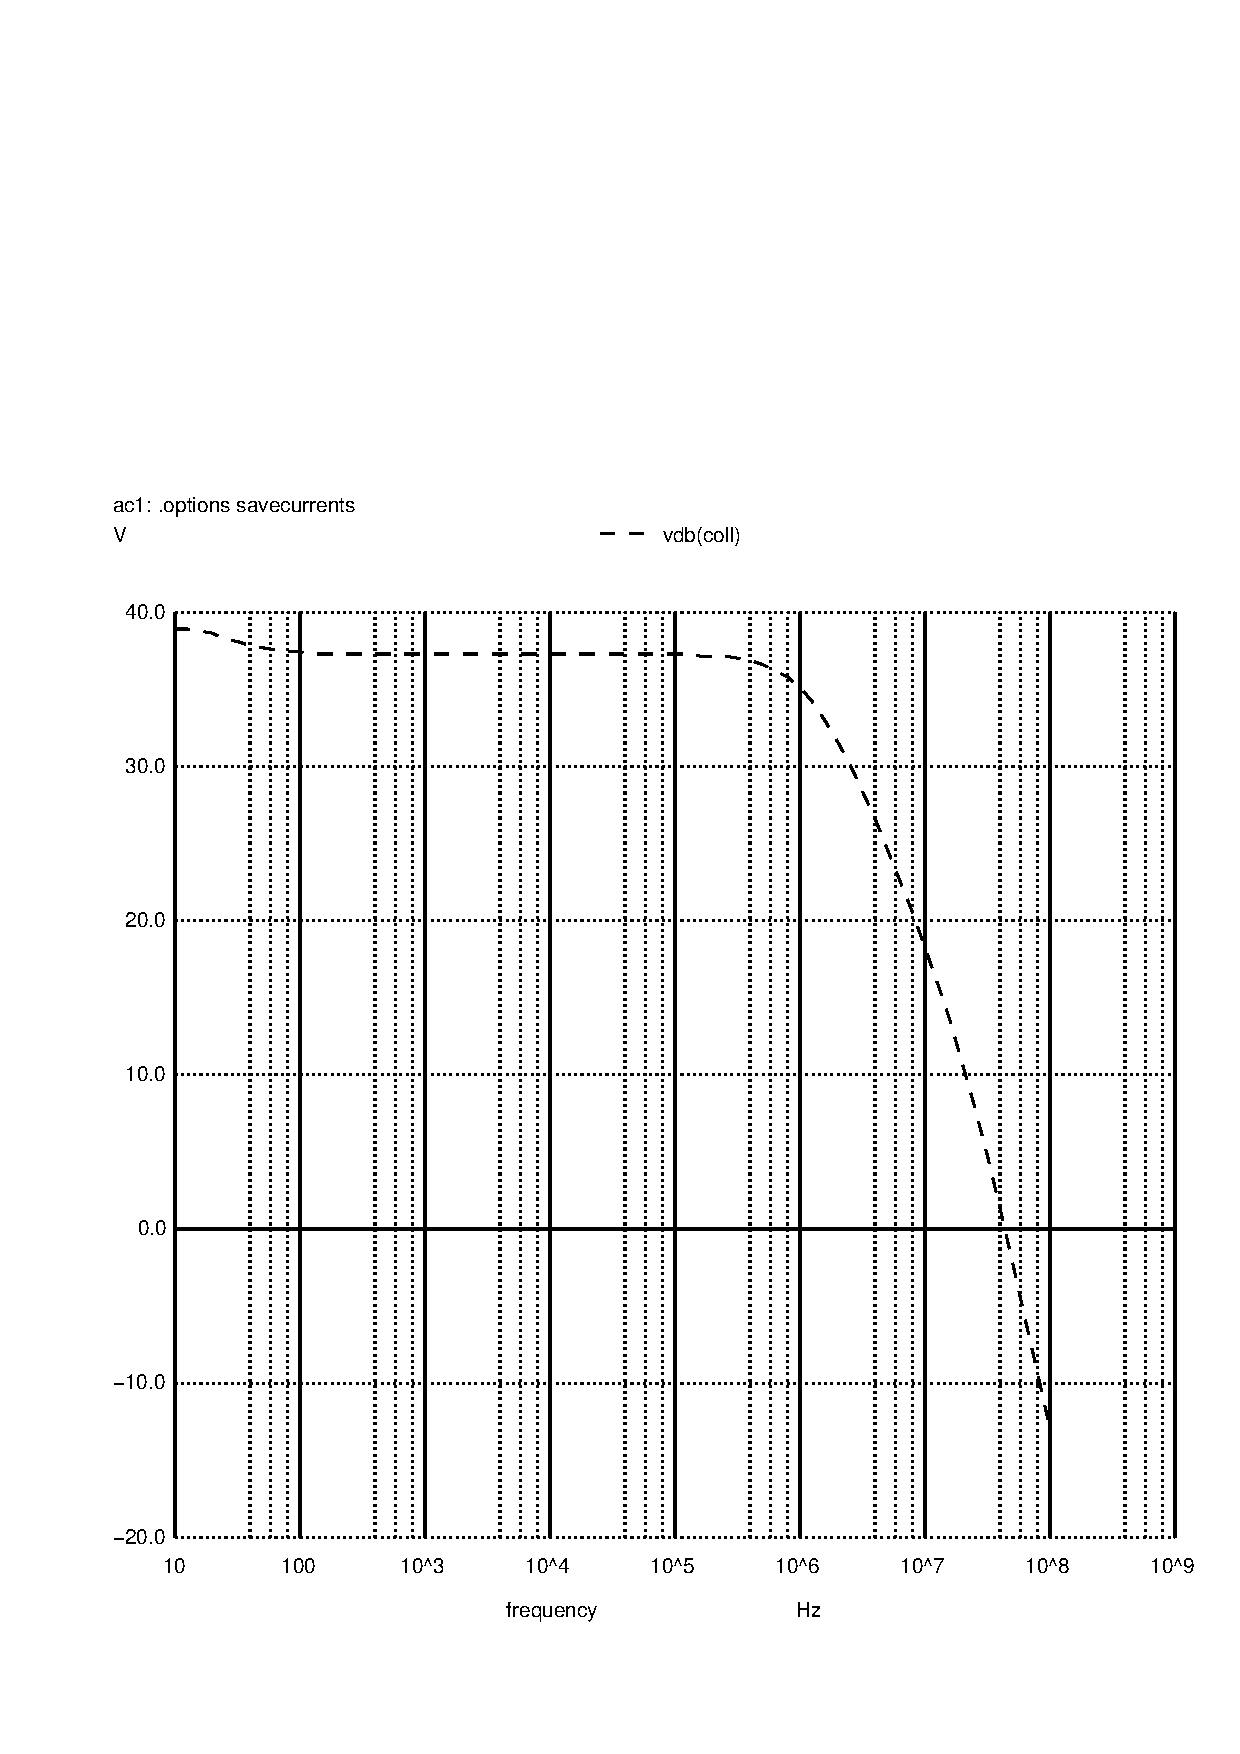
\includegraphics[width=.75\linewidth]{vo1f.pdf}
  \caption{Input Voltage}
  \label{fig:sim4}
\end{subfigure}%
\begin{subfigure}{.5\textwidth}
  \centering
  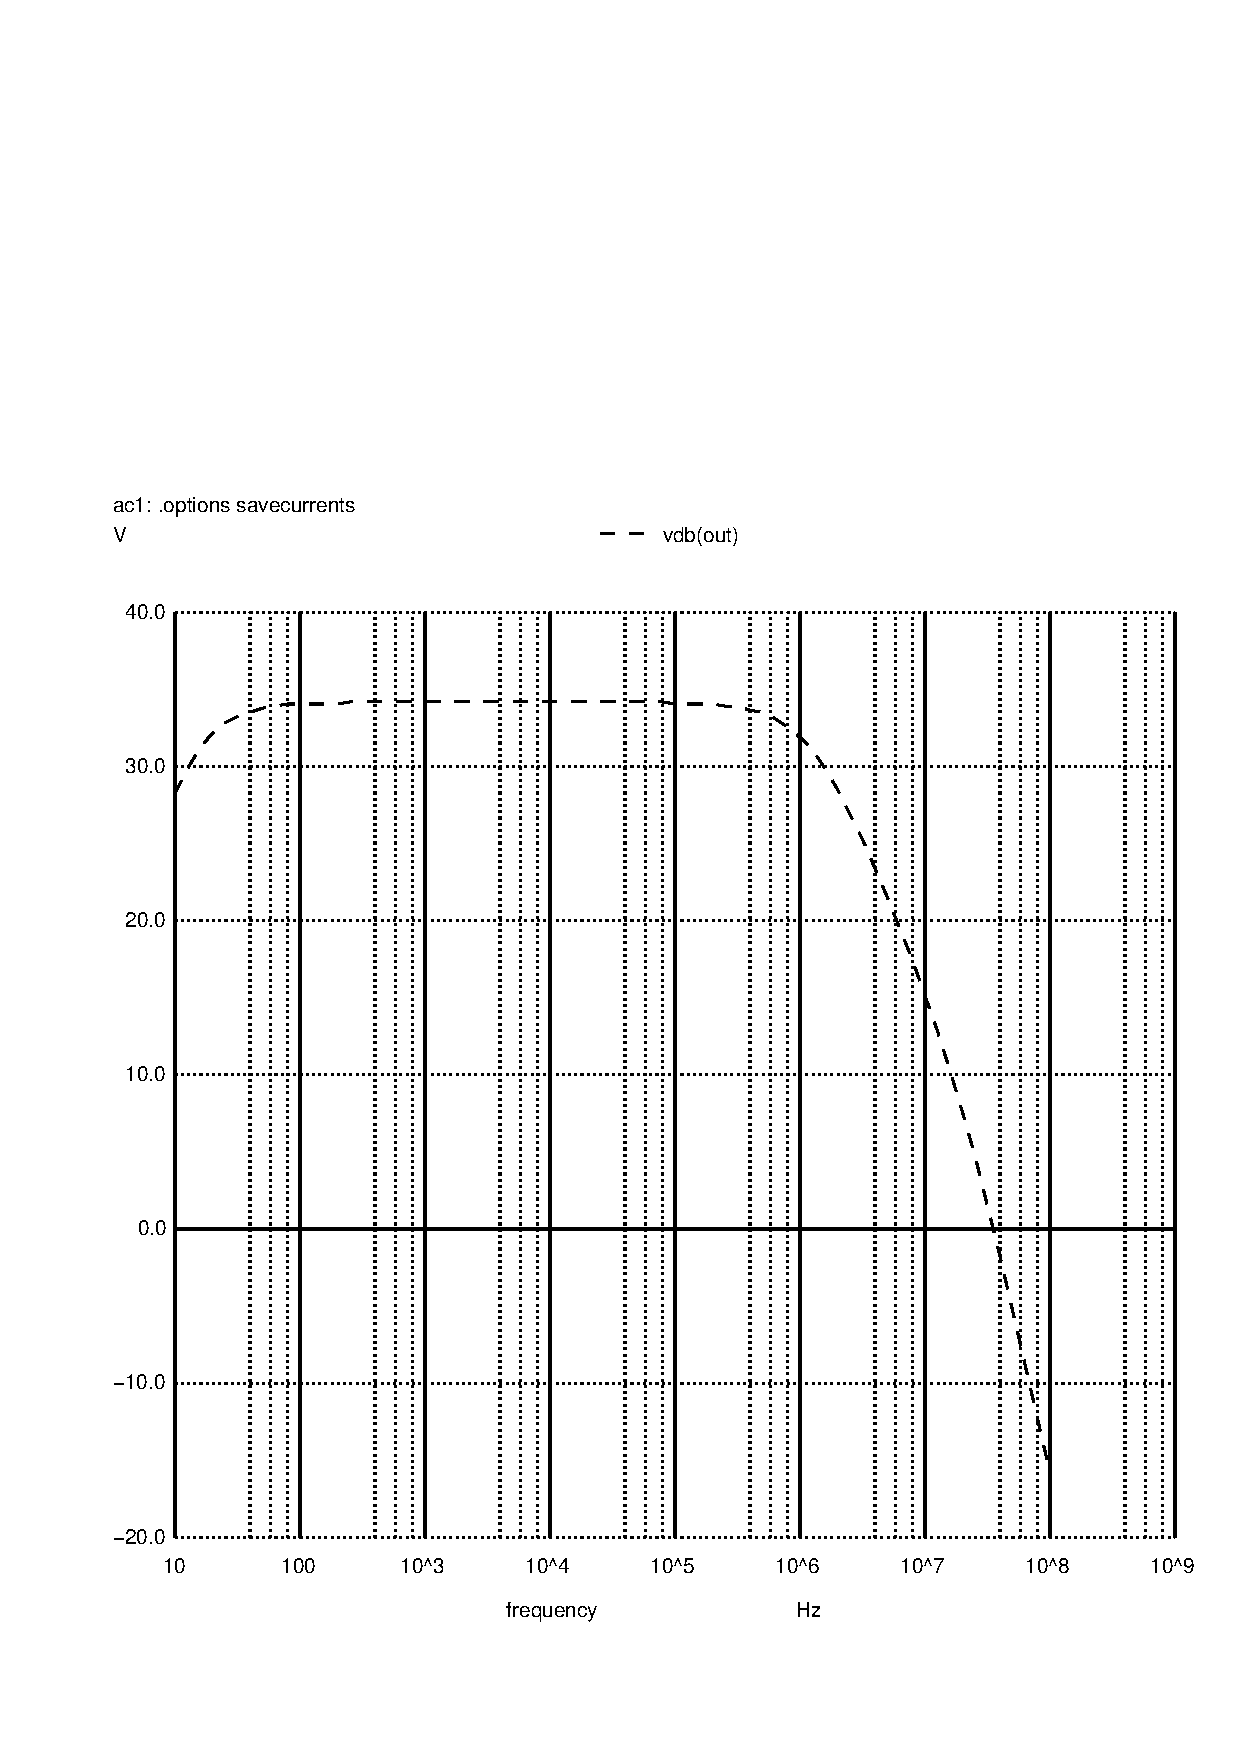
\includegraphics[width=.75\linewidth]{vo2f.pdf}
  \caption{Output voltage}
  \label{fig:sim5}
\end{subfigure}
\end{figure}

\subsection{Input and Output Impedances}
\par Next, the input and output impedances were calculated as seen on the tables below,

\begin{table}[h]
  \centering
  \begin{tabular}{|l|r|}
    \hline    
   Zin & -1445.61 + 303.661 j\\ \hline

   \end{tabular}
  \caption{Input impedance ($\Omega$)}
    \label{tab:ZI}
\end{table}

\begin{table}[h]
  \centering
  \begin{tabular}{|l|r|}
    \hline    
   Zo & 25.852 + 1.292 j\\ \hline
Zo(int) & 25.8843\\ \hline

   \end{tabular}
  \caption{Output impedance ($\Omega$)}
  
  \label{tab:ZO}
\end{table}

\par As we can see, the input impedance is higher than the outup impedance. This plays well to maximise the gain as the voltage in node in2 needs to be as close to Vin as possible, reducing the losses. To do that, as we can see in the voltage divider formulae, it's necessary to increase the resistance value. The opposite logic is used to the output impedance. Again, considering the voltage divider formulae, the output impedance must be as small as possible to guarantee the maximum output voltage and gain. Even though the output impedance should be lower than the $8\Omega$ to maximise the output voltage, because of the different parameters in the merit formula, our otimization made the value higher than the optimal value if it was the only one. 

\subsection {Cost and Merit}
\par Finally the cost and merit of the circuit described and seen in the images before  is calculated in ngspice. The results are shown on the table as it follows.

\begin{table}[ht]
  \centering
  \begin{tabular}{|l|r|}
    \hline    
   V Gain&34.1403\\ \hline
Low Cut Off Freq& 15.8089 Hz\\ \hline
High Cut Off Freq& 1.22341E+06 Hz\\ \hline
Bandwidth&1.22339E+06 Hz\\ \hline
Cost & 2198.94 MU\\ \hline
merit & 1201.48\\ \hline

   \end{tabular}
  \caption{Cost and Merit of the circuit}
  \label{tab:cost}
\end{table}


\newpage
\section{Comparison}
\label{section:comparison}

\par Now a comparison between the theoretical analysis and the experimental analysis results of the gain is done. In the previous sections, for the theoretical analysis an operating point analysis was performed and the values obtained. The table \ref{tab:op} shows the values obtained and compares them.

\par As we can see there are some errors associated with the theoretical model when compared to the experimental results, especially for the values of the voltage in the nodes.
Nosso
********************************
TEKAs



In the Ngspice table, the only parameters in comparison are $@q1[ib]$, $@q1[ic]$, $@q1[ie]$, $base$, $coll$ and $emit$.
\par As one may observe, some discrepancies in the voltage values are noticeable. Nevertheless, the values of the currents flowing are are within reasonable intervals of similarity. Therefore, the gain computed in Octave should not be severely affected by this. It is important to highlight that the theoretical gain expression is dependent on the value of the current $I_{C}$ because of the incremental parameter $g_{m}$. 

\par Aditionally, the gain, bandwidth and cut off frequency results were also computed. As predicted, the voltage gain in the theoretical approach is greater than in the Ngspice computation. Moreover, since we do not have the theoretical high cut frequency, we can only compare the results for the low cut frequency, which are very similar as far as the order of magnitude is concerned. For this reason, as the bandwidth is the subtraction between high and low cut frequencies, it should not be compared.










\newpage
\section{Conclusion}
\label{sec:conclusion}

\par In this laboratory assignment, the goal of conceiving an AC/DC converter was achieved. As seen in the whole report, the theoretical results (obtained using Octave) didn't exactly match the simulated ones (obtained using NGspice) because of the non-linearity of the diodes (as predicted), but overall the final result was pretty decent and it's good enough to validate the model used in the theoretical analysis.




%\cleardoublepage

% ----------------------------------------------------------------------
%  Bibliography
% ----------------------------------------------------------------------
%\addcontentsline{toc}{section}{\bibname}
%\bibliographystyle{abbrvunsrtnat} % <<<<< SELECT IF USING REFERENCES BY NUMBER (CITATION ORDER)
%\bibliography{../../../BIBfile.bib}

% ----------------------------------------------------------------------
\end{document}
% ----------------------------------------------------------------------







